%%
%%       --- a chapter ---
%%
%% A chapter

\chapter[Introduction]{Introduction}\label{ch:introduction}

One of the most remarkable achievements in physical sciences over the last few decades is the precision to which cosmologists have been able measure the initial conditions of our Universe. We know very well how it all began 13.8 billion years ago and what the starting ingredients were. From the panoply of planets, stars and galaxies we see around us today, we also have a good grasp on what those ingredients eventually became. The challenge facing Astronomy is to fill in the gaps in that long history and shed light upon the underlying physics which shaped the formation and evolution of these celestial objects.

\section{The Early Universe}
What makes the measurements of the initial conditions in our Universe possible is the detailed observation of the cosmic microwave background (CMB). Famously discovered accidentally by Arno Penzias and Robert Wilson in 1964 \citep{Penzias:1965es} but independently postulated several times in the preceding decades, the CMB represents the oldest light in the Universe. For the first $\sim 373,000$ years after the Big Bang all baryonic matter in the Universe -- including free electrons, protons and neutrons -- was coupled together in a hot, uniform, radiation-filled hydrogen plasma. As the Universe expanded and cooled, the electrons and protons eventually cooled enough to form neutral atoms (`recombination') shortly before cooling far enough to allow the radiation field to decouple from the baryons and the photons to stream freely through space (`decoupling'). It is those primordial photons that have been propagating through space and slowly cooling until this date to produce the cosmic microwave background we observe today.

Since the initial measurements of the CMB 50 years ago, a succession of ground-based, balloon-borne and space-based telescopes have measured the CMB with increasing precision. Despite initially appearing uniform in all directions, in 1992 data from the Cosmic Background Explorer (COBE) satellite indicated minute variations in the temperature of the CMB on small scales\footnote{Re-analysis of data from the Soviet RELIKT-1 anisotropy experiment did in fact lead to publication of anisotropy results several months before the COBE announcement (re-published in \citeauthor{Strukov:1992ua}~\citeyear{Strukov:1992ua}). However it was the COBE results for which the Nobel prize was later awarded.}. These anisotropies have since been measured to exquisite precision by the Wilkinson Microwave Anisotropy Probe (WMAP) and Planck experiments, leading to strong support for the currently favoured model of $\Lambda$-Cold Dark Matter (\cdm{}) cosmology. Figure~\ref{fig:cmb_comparison} illustrates just how much each new generation of space-based CMB laboratory has improved our picture of the microwave background.

\begin{figure}[!hb]
	\centering
	\includegraphics[width=0.9\textwidth]{CobeWmapPlanckComparison.jpg}

	\vspace{0.5in}
		
	\includegraphics[width=0.8\textwidth]{Planck_CMB.jpg}
	
	{\sffamily Planck CMB}
	\caption[The Cosmic Microwave Background anisotropy.]{Top: Illustration of the increase in angular resolution offered by successive generation of CMB observatories, Credit -- NASA/JPL-Caltech/ESA. Bottom: The all-sky map of the cosmic microwave background anisotropies as measured by the Planck satellite, Credit -- ESA and the Planck Collaboration.}
	\label{fig:cmb_comparison}
\end{figure}

Imprinted by primordial quantum fluctuations that have grown and stretched with the expansion of the Universe, the observed anisotropies carry a wealth of information and any candidate cosmological model must be able to explain their properties. The current `standard' \cdm{} cosmology (constrained by the Planck measurements) tells us that the present Universe is one consisting of precisely $30.89 \pm 0.62\%$ matter with the rest ($69.11 \pm 0.62\%$) comprised of an unknown `dark energy', denoted `$\Lambda$' \citep{2015arXiv150201589P}. Of that $\sim 30\%$ matter, only a modest $\sim 5\%$ is baryonic matter, visible as stars, dust and gas in the inter-stellar and intergalactic medium (ISM and IGM respectively). The remaining  $\sim 25\%$ of matter is cold dark matter (CDM), itself still very much a mystery.

In the \cdm{} model, the primordial fluctuations that gave rise to the CMB anisotropy and cold dark matter also play a crucial role in the formation of structure in the Universe. Before recombination occurred, the primordial elements which formed through big bang nucleosynthesis (BBN; \citeauthor{Burles:2001kr}~ \citeyear{Burles:2001kr}) were coupled to the electromagnetic radiation field through Thomson scattering; smoothing out any inhomogeneities. However, the non-baryonic dark matter was completely decoupled from the electromagnetic radiation and able to form small over-densities around the tiny density fluctuations. Under the force of their own gravity, these small over-densities were able to collapse into larger halos. Meanwhile, because of the radiation pressure on the coupled baryon-photon plasma the `ordinary' matter was prevented from collapsing. It was not until recombination and the baryon-photon decoupling occurred that the baryons were able to fall into the gravitational potentials created by the collapsed dark-matter halos.

Over the following few hundred million years these over-densities continued to grow in a so-called hierarchical way, whereby the first halos to collapse were small and larger halos were built up through many mergers of smaller halos. Eventually, the baryonic matter in the centre of the deepest gravitational potentials reached a high enough density and the neutral gas reached such high temperatures and pressures that the molecular hydrogen was able to radiate energy away. By radiatively cooling, the dense baryonic potentials could collapse further and reach high enough pressures and temperatures for nuclear fusion to commence; forming the first stars. The exact process of how these first stars formed is not well known and represents one of the true frontiers of modern astronomy \citep{Bromm:2013dk}. However, what is for sure is that these first stars signalled the end of the so-called `dark ages'.

With the formation of the first stars and their emission of energetic photons into the surrounding medium, the previously neutral hydrogen of IGM began to ionize into the predominantly ionized medium we see around us today. This era is known as the epoch of reionization (EoR). By using the imprinted polarisation on the CMB, WMAP and now Planck have been able to measure the total optical depth to the surface of last scattering, revealing that the start of the process of reionization (averaged across the Universe) began around 560 million years after the Big Bang \citep{2015arXiv150201589P}.

However, the details of the epoch of reionization remain something of a mystery and have been important drivers in both the study of cosmology and galaxy evolution. For example, which were the sources that powered reionization? What form did the transition take, was it a longer drawn out process or did it occur in one (or more) rapid transition? Were there enough galaxies to provide the required number of ionizing photons, or were quasars or exotic stellar populations required? 
 
\section{Galaxy Formation}\label{sec:intro-galform}

If the CMB represents constraints of the initial conditions on the time evolution of galaxies, observations of the local evolved galaxy population are effectively the corresponding boundary condition at late times. Any theory or description of galaxy formation and evolution must have as its goal the ability to explain both the wide range of galaxy properties that exist and the correlations and links between many of those properties.

The most obvious and earliest property to be categorised and studied was the morphology of galaxies -- their visual appearance. The morphology of local galaxies falls broadly into two categories: ellipticals and spirals, famously first visually classified by Edwin Hubble \citep{Hubble:1926be}. Elliptical galaxies as the name suggests are ellipsoidal and supported predominantly by the random motions of their stars (dispersion dominated). In contrast, spiral galaxies are flatter disc-like structures, supported mainly by their rotation and usually containing one or more visible spiral arms (hence the term `spirals') which themselves may or may not include a barred structure. The majority of local galaxies sit somewhere between these two types, with the elliptical component commonly referred to as the `bulge' and the flat rotational structure known as the `disc'. In Hubble's eponymous `tuning fork' diagram, galaxies lie on a sequence from entirely bulge-dominated elliptical galaxies through to pure discs with a mixture of the two components in between.

However, not all galaxies can be placed neatly along the Hubble sequence (or other such updated scheme, \citeauthor{deVaucouleurs:1959vq}~\citeyear{deVaucouleurs:1959vq}). Firstly, there are peculiar or irregular galaxies, which resemble neither ellipsoids nor discs due to the presence of features such as multiple subcomponents, long tail-like features and distorted structures. Many of these peculiar features have been associated with interactions or mergers with other nearby galaxies, suggesting that these interactions perhaps play a role in transforming one morphology into another. Secondly, a subset of irregular galaxies are those known as dwarf irregulars, galaxies that have low masses and large amounts of gas and on-going star formation, potentially representing local analogs of the earliest galaxies. 

In addition to the wide diversity of galaxy morphologies, local galaxies span a wide range in luminosity and stellar mass (several orders of magnitude). Furthermore, not only do overall galaxy luminosities vary, they come in a wide range of colours (the ratio of luminosities or fluxes in two different photometric filters), which appear to be linked to the morphological type. Early-type galaxies (including ellipticals and lenticulars) generally have redder colours than late-type galaxies (spirals and irregulars), i.e. the luminosity in the longer wavelength filter is high relative to that in the shorter `bluer' filter\footnote{There are caveats to this statement, in that the reddening of galaxy colours by the attenuation of dust must also be taken into account. Section~\ref{sec:intro-sed} of this introduction explores in more detail the processes and difficulties of measuring galaxy properties through their colours.}. This bi-modality is particularly well illustrated by the galaxy colour-magnitude (or colour-mass) diagram, an example of which is shown Figure~\ref{fig:colour_mass}.

\begin{figure}
\centering
	  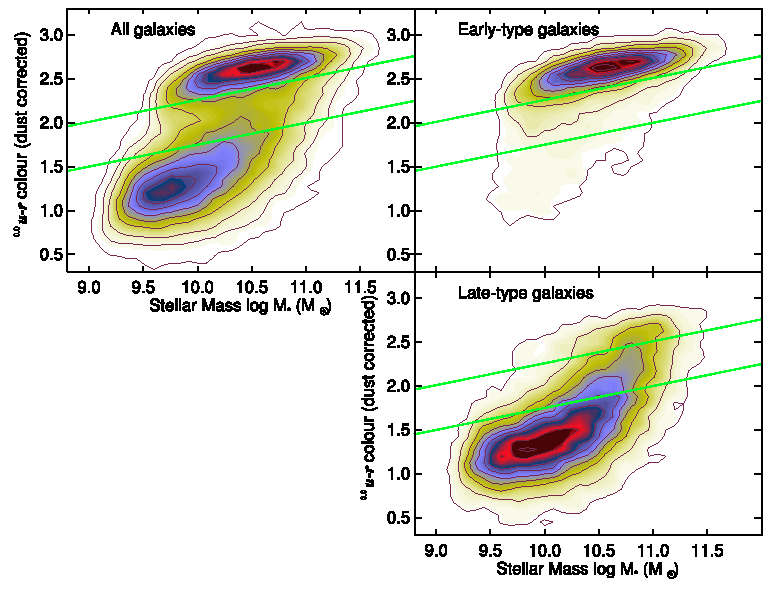
\includegraphics[width=0.95\textwidth]{ColourMass_Schawinski.pdf}
	  \caption[Colour ($\mathcal{U} - \mathcal{R}$) vs stellar mass for nearby galaxies from the SDSS all-sky survey, separated by visual morphological classifications done through the Galaxy Zoo project.]{Colour ($\mathcal{U} - \mathcal{R}$) vs stellar mass for nearby galaxies from the SDSS all-sky survey, separated by visual morphological classifications done through the Galaxy Zoo project. In the left-hand panel the `red sequence' and `blue cloud' are clearly visible in the top and bottom concentrations of galaxies respectively. Separating the galaxy by morphological type further reveals the correlation between colour and morphology, with early-type galaxies (elliptical or bulge dominated) being red and typically more massive and late-type (spiral or disc dominated) being blue and of lower mass. Figure from \citet{Schawinski:2014ep}.}
	  \label{fig:colour_mass}
\end{figure}

Since the colour of a galaxy is intrinsically related to the age of its stellar population, the observed bi-modality is indicative of differences in the formation histories between early and late-type galaxies. More specifically, redder galaxies are generally older and/or more chemically enriched than bluer galaxies. The early-type galaxies that make up the red sequence must therefore have built up their stellar mass and ceased star-formation earlier (on average) than the late-type galaxies which make up the blue cloud. The idea that the most massive galaxies formed first and quickest is known as `downsizing' \citep{Cowie:1996fb}, and at first seems contrary to what would be expected in the simple hierarchical structure formation models, whereby the largest galaxies would be formed later in cosmic history through the merging and build-up of many smaller galaxies \citep{DeLucia:2006gl}.

One of the primary aims of modern astronomy is to understand how this bi-modality was formed, and what physical processes governed the evolutionary pathways of these different galaxy types. By studying in detail the stellar populations, chemistry and kinematics of local galaxies, it is possible to work backwards to understand their histories. However, the beauty of a Universe in which light has a finite travel time is that we are able to peer back through cosmic history and see these processes in action, providing a direct view of galaxy formation and evolution at earlier times. 

\begin{figure}
\centering
	  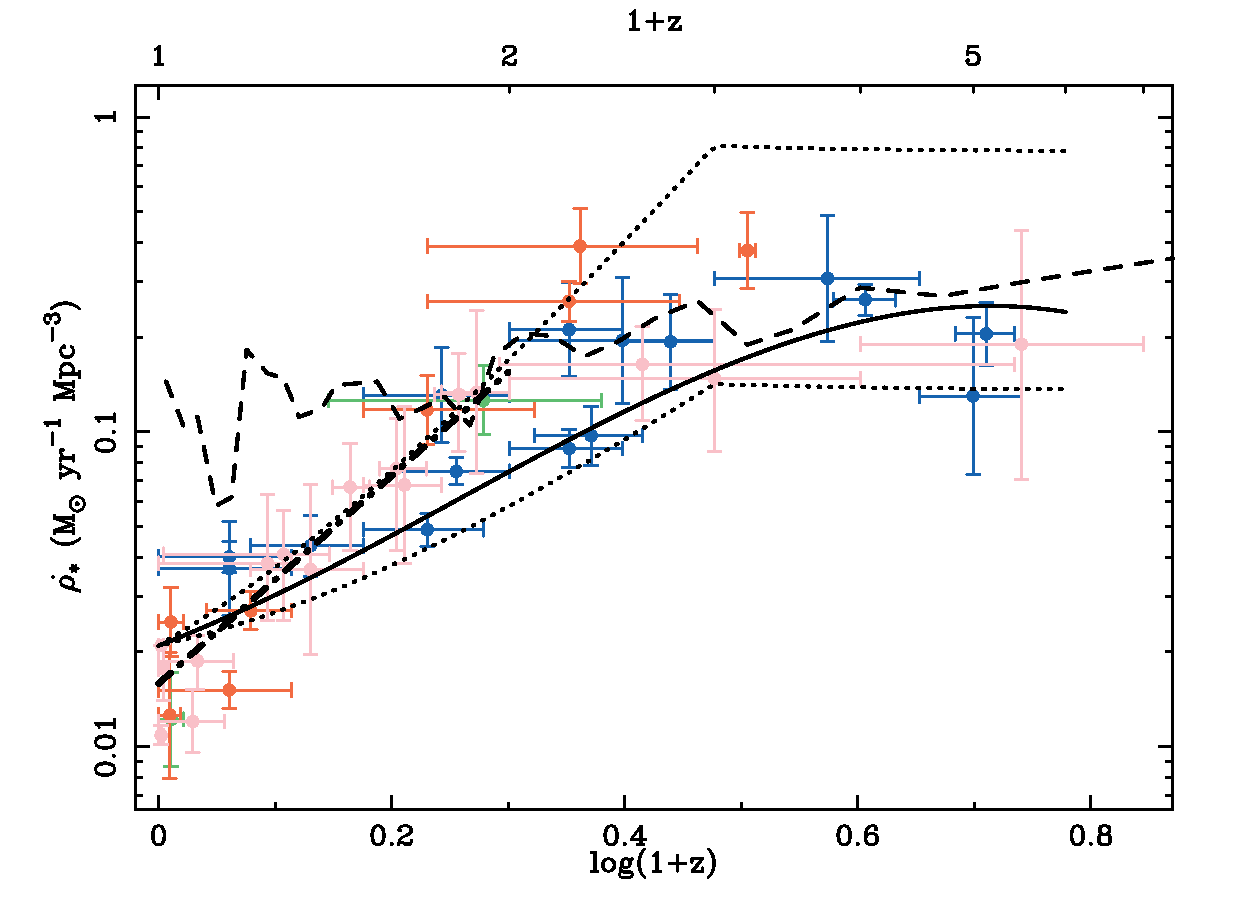
\includegraphics[width=0.95\textwidth]{Hopkins2004.pdf}
	  \caption[Evolution of the star-formation rate density through cosmic time.]{Evolution of the star-formation rate density through cosmic time. Data points are colour-coded corresponding to the star-formation rate indicator, with UV (blue), $[\rm{O}\textsc{ii}]$ and H$\alpha$/H$\beta$ (green and red respectively) and Xray/far-infrared/sub-millimetre and radio estimates (pink). The dot-dashed line at $z<1$ shows the best-fitting line to the collective data. The solid and dotted lines show estimates additional radio based SFR estimates while the long-dashed line shows the `fossil' record from local group galaxies. Figure from \citet{Hopkins:2004eu}, see references therein for individual SFR density citations. }
	  \label{fig:hopkins04}
\end{figure}

Observations of the star-formation rate density indicate that the star-formation history of the Universe peaked at around two to three billion years after the Big Bang at a redshift of $2 \lesssim z \lesssim 3$ (Figure~\ref{fig:hopkins04}), indicating that the majority of stellar mass in galaxies was formed more 6 Gyr ago. Studies of galaxy morphologies through time have also shown that the Hubble sequence began to form in the few billion years following this peak in star-formation \citep{Mortlock:2013dg}.

In addition to extensive study of galaxy star-formation rates and stellar masses since the epoch of peak star-formation (sometimes dubbed `Cosmic high-noon'), much work has also gone into measuring the merger history of galaxies across time. By studying the statistics of galaxies in close pairs \citep{Patton:2000kt,LeFevre:2000iq,Bell:2006ey,Bluck:2009in,Bluck:2012dh} and the fraction of galaxies which show signs of morphogical disturbance due interactions with nearby companions \citep{Conselice:2003jz,Conselice:2008de,Lotz:2011bu}, the merger rates of galaxies have been well studied as far back as $z\sim3$. Extending such analysis to earlier epochs and to lower mass galaxies has however proved difficult, with very few even attempting to do so \citep{2009MNRAS.397..208C}.

As mentioned previously, one of the key predictions for structure formation in a \cdm{} universe is that mergers play a vital role in the formation and evolution of galaxies. Furthermore, mergers are also a potential driver for evolution in other galaxy properties such as their structure, kinematics and morphology \citep{Conselice:2014ct}. Between the peak in the cosmic star-formation history and now, the progenitors of today's most massive galaxies grew through almost equal parts of star-formation, major mergers and minor mergers \citep{Ownsworth:2014gt}. Understanding how those galaxies assembled before that time represents one of the current challenges in extragalactic astronomy.

It is also thought that major mergers, and in particular mergers between gas-rich galaxies, may be important in fuelling the growth of central super-massive black holes of galaxies \citep{Springel:2005co,Hopkins:2008ip,Hopkins:2008gr}. Measuring the abundances of gas-rich mergers through time is therefore essential in linking them to the rise and fall of AGN and starburst activity through cosmic history.

In Chapters~\ref{ch:smf} and \ref{ch:mergers} of this thesis, we aim to better understand how those progenitors grew into what we see at $z=3$ through studying the stellar mass growth, star-formation rates and merger histories of galaxies during the first few Gyr of galaxy formation. Until recently, the ability to find and observe galaxies as far back as the first two billion years of the Universe was just not possible. In the last two decades however, huge leaps in both the technology and observational techniques has allowed for remarkable progress in studying the first galaxies.

\subsection{Illuminating the dark ages}\label{sec:intro-distant-galaxies}
The first realisation that galaxies could be observed at truly cosmological distances was made by Maarten Schmidt who measured the redshifts of five quasi-stellar objects (QSOs) out to $z\approx 2$ \citep{Schmidt:1965gm}. These QSOs, or quasars, are now better understood to be the emission from accretion onto the super-massive black holes at the centre of galaxies. At the time of these measurements, their properties were still very a much a mystery. 

Around this time, \citet{Partridge:1967iw} made the first predictions of the potential to detect normal star-forming galaxies at early times through their bright Ly-$\alpha$ emission, the UV continuum emission and the Lyman absorption decrement. All UV bright galaxies exhibit a characteristic drop at 912$\rm{\AA}$ (the ionization energy of neutral hydrogen) and in young star-forming galaxies rich in cold gas (and hence neutral hydrogen) this break was expected to be very strong. It was therefore hoped that such a strong spectral feature provide an excellent way of identifying high-redshift galaxies. Despite valiant attempts along the way \citep{Meier:1976ch}, it would be several decades before such searches became successful. 

By using a carefully selected set of optical filters, \citet{1992AJ....104..941S} were able to successfully select an ordinary star-forming galaxy at $z\sim 3.4$ based on the photometric colours of filters either side of the redshifted Lyman absorption decrement at $z\sim3$. This technique, now commonly known as Lyman break selection, made it possible to easily select galaxies at high redshift with a good degree of reliability using only photometric surveys. 

\begin{figure}
\centering
	  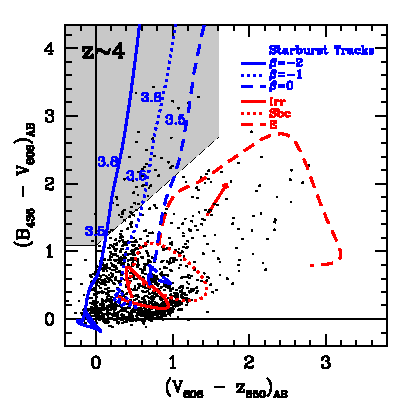
\includegraphics[width=0.7\textwidth]{BouwensCuts.pdf}
	  \caption{Two-colour diagram illustrating selection criteria used to select $z\sim4$ (`$B$ dropouts') in the Hubble Ultra Deep field by \citet{Bouwens:2009ik}. The blue solid, dotted and dashed lines illustrate the colour tracks as a function of redshift for galaxies with UV continuum slopes of $\beta = -2$, $-1$ and 0 respectively. The red lines show the comparable tracks for standard morphological types at lower redshift.}
	  \label{fig:colourcuts}
\end{figure}

In contrast to the relative stagnation of the preceding two decades, the subsequent years have seen a relentless and rapid progression in the study of galaxies at high-redshift. Following the first few detections through the Lyman break technique, the \emph{Hubble} Deep Field allowed this technique to applied further, to redshifts of $z\sim4$ and beyond \citep{Steidel:1995kx,1996MNRAS.283.1388M} (see Figure~\ref{fig:colourcuts} for an example of the colour criteria used to select such galaxies). Spectroscopic confirmation of the brightest $z\sim3$ Lyman break galaxies soon followed \citep{Steidel:1996jd}. During this time, the first successful detection of high-redshift galaxies through their Ly-$\alpha$ emission line were also made \citep{Hu:1996eq, Hu:1998uh, Cowie:1998dt}, finally confirming the predictions of \citeauthor{Partridge:1967iw}. 

Now proven successful, the availability of deep optical data from both ground and space based instruments meant that the selection of high-redshift galaxies could be extended both to fainter samples and out to even higher redshifts ($z\sim6$) both photometrically \citep{1999ApJ...519....1S, Thompson:2001da, Thompson:2003dp, Fontana:2003ch, Stanway:2003fx, Giavalisco:2004et, Dickinson:2004ba, Capak:2004im} and spectroscopically \citep{Bunker:2003hc,Stanway:2004kr,Stanway:2004gu}. At $z\simgreat 6.5$ the Lyman break has been redshifted out of the optical wavelengths into the near-infrared regime ($\lambda \sim 1\mu$m) where observations deep enough to make strong detections of galaxies above the break at $z\sim7$ were much more difficult, although not impossible \citep{Bouwens:2004gn}. There was however a limit to how far this method could be pushed with the existing ground and space-based facilities, temporarily putting the rush to ever higher redshifts into a somewhat lower gear (for now).

The installation of the Wide-field Camera 3 (WFC3) on the \emph{Hubble Space Telescope} in spring 2009 came as a particular boon to the study of detection of galaxies at $z\sim7$ and beyond. With a significantly more sensitive near-infrared detector, as well as an improved filter set and increased field-of-view compared to the previous NICMOS camera, the earliest data taken with the WFC3/IR camera allowed several independent groups to find robust samples of galaxies at $z\sim7$, deep into the epoch of reionization \citep{Bunker:2010gx, Finkelstein:2010fw, 2011A&A...532A..33G, Labbe:2010ho,2010ApJ...709L..21O,2012ApJ...759..135O,Bouwens:2010dk,2011ApJ...737...90B}. The greatly improved survey efficiency has also meant that large-scale \emph{Hubble} projects such as CANDELS \citep{2011ApJS..197...35G} and 3D-HST \citep{Brammer:2012bu} are now able to make deep near-infrared surveys over far wider areas than possible with NICMOS. In Section~\ref{sec:intro-candels} we present further details of the CANDELS survey and its aims.

Alongside the advances in space based near-infrared observations has also come advances in the sensitivity of ground-based telescopes. Although not able to reach the same depths as those possible with WFC3, the wider field of view means that deep ground-based surveys such as UltraVISTA \citep{McCracken:2012gd} or the UKIDSS Ultra Deep Survey \citep{Lawrence:2007hu,Cirasuolo:2007bz} can survey far larger areas ($>1 \rm{deg}^{2}$) than HST and allow for searches of the brightest but rarest sources at $z > 4$ \citep{McLure:2006fg,2009MNRAS.395.2196M,2010A&A...524A..28C}.

It is not just at the most extreme redshifts for which the addition of deep near-infrared observations have been of benefit. With an increase in the number of optical and infrared filters has also come an increase in the use of photometric redshift selection in place of the traditional colour-colour Lyman break selection \citep{McLure:2006fg,McLure:2010hq}. Photometric redshift analysis typically works by fitting a set of known template spectra (either empirical or model generated) to the full range of broadband filters available for a galaxy in order to find the redshift that minimises $\chi^{2}$ \citep{Bolzonella:2000uw,Brammer:2008gn} or maximises some Bayesian likelihood \citep{Benitez:2000jr}\footnote{Other more novel approaches such as the use of artificial neural networks \citep{Collister:2004fx} have also been applied but have not gained such widespread usage.}.

The estimation of photometric redshifts is strongly dependent on the ability of the method to identify key spectral features in the observed data, especially the main Balmer and Lyman spectral breaks. In this regard, the use of photometric redshifts to select galaxy at $z > 3$ is not far removed from Lyman break selection. However, the benefit of photometric redshift analysis is that it is able to take into account the shape of the galaxy spectrum above the break and at other points in the spectrum to discern between similar spectral features which would otherwise be degenerate in a single colour. Perhaps more importantly, photometric redshifts also make it possible to quantify the uncertainty in identifying these spectral features in a way that a binary yes-or-no colour selection cannot (e.g. \citeauthor{Dunlop:2007fo}~\citeyear{Dunlop:2007fo}). In Chapter~\ref{ch:smf} of this thesis, we investigate the potential discrepancy between the two selection methods at high-redshift and illustrate the advantages of photometric redshifts when sources suffer from significant photometric scatter.

It is worth noting that the selection of high-redshift galaxies through their rest-frame UV emission is no longer the only option. Developments in detectors of all types has led to galaxies at $z > 3$ being found through their rest-frame optical and near-infrared \citep{Franx:2003cx,vanDokkum:2003bl} and sub-mm/far-infrared \citep{Walter:2003ul,Robson:2004gu} emissions and via gamma-ray bursts \citep{Haislip:2006gx,Kawai:2006kk,Tanvir:2009gq}.

\subsubsection{Sample contamination}
While there now exist several methods for selecting high redshift galaxies from large photometric catalogs, it is also vitally important to take into account the range of other (non-) astrophysical sources which can also satisfy high redshift selection criteria. Potential contaminants for high-redshift galaxy samples can broadly be separated into types; each corresponding to a different scale within the Universe.

Firstly, there is local or instrumental contamination to contend with. When pushing the selection of galaxies to the very limits of its current detection capabilities, cosmic rays or image artefacts in \emph{Hubble Space Telescope} (HST) photometry can have an increased effect on the generation of spurious sources in catalogs. In any single HST photometry exposure, numerous pixels within the CCD detector will be hit by cosmic rays passing through the telescope resulting in bright over saturated pixels in otherwise empty areas of the sky. 

For the vast majority of circumstances, such cosmic ray hits are not a problem. Since the distribution of affected pixels is entirely random, by taking multiple exposures it is much easier to identify the effected pixels and exclude (or `mask') them from the final reduced images. Furthermore, if such a spurious source is missed by these cosmic ray rejection algorithms (e.g. \citeauthor{vanDokkum:2001go}~\citeyear{vanDokkum:2001go}) and results in a statistically significant detection in the resulting photometry catalog, the lack of any source detection in other photometric bands will serve to identify the source as contamination. However, if no such detection in any other photometric band is actually expected (as is precisely the case for potential $z\sim 10$ to 12 galaxies), such spurious sources pose a genuine problem and must be considered carefully \citep{Bouwens:2011el}. Taking the potential detection of a $z\sim10$ galaxy by \citet{Bouwens:2011el} as an example, the non-spurious nature of the detection was determined by confirming its detection in two independent subsets of the data (i.e. exposures taken in different years). Such a confirmation does not necessarily mean that the object in question is definitely at high redshift \citep{Brammer:2013dg} but it can at least rule out that source as a spurious detection.

A second major source of potential contamination is low-mass stars within the Milky Way itself \citep{Caballero:2008ea}. For low-mass stars, the combination of a cool blackbody temperature for the underlying stellar emission and strong absorption lines within their atmospheres (e.g. TiO, H$_{2}$O, CH$_{4}$) can combine to produce broadband photometric colours which are very similar to those of galaxies at $z \gtrsim 6$ \citep{Finkelstein:2014ub,Wilkins:2014jp}. The classification of objects as stars (and their exclusion from high-redshift galaxy samples) is most difficult for ground-based observations, where the larger point-spread function makes separating compact distant galaxies from stellar point sources more difficult \citep{Bowler:vl,Bowler:2013wz}. However, even for observations with high resolution HST photometry, it is still necessary to use additional information such as photometric colours or spectroscopy to discriminate between stellar and extragalactic sources \citep{Stanway:2008fj,Pirzkal:2009cg}.

Finally, other extragalactic sources can also pose problems in creating clean and robust samples of galaxies at $z>3$. For photometric selection of high-redshift galaxies, dusty red galaxies at lower redshifts can cause significant confusion in the selection methods and can be a major source of contamination. The confusion occurs due to the similarity in colours between the Lyman break at high redshift and a Balmer/4000$\rm{\AA}$ break with strong dust attenuation (at $\approx 3 - 5\times$ lower). It is precisely this confusion between spectral features which the inclusion of long wavelength \emph{Spitzer} data in photometric redshift fitting is intended reduce \citep{2011MNRAS.418.2074M}.

A second class of potential low-redshift galaxy contaminants are extreme-emission line galaxies (EELGs) at $z > 1$ \citep{vanderWel:2011ch,Atek:2011ka}. Although they do not strongly affect most photometric selection methods they do pose a problem when searching for high redshift galaxies via their Lyman-$\alpha$ emission or when looking for Lyman break drop-outs at the very highest redshifts \citep{Brammer:2013dg}. EELGs have been found to be low-metallicity dwarf galaxies which are undergoing starbursts, resulting in optical emission lines (e.g. $\left [\rm{O}\textsc{iii} \right]$) with extreme equivalent widths and faint continuum photometric detections similar to those expected for high redshift Lyman-$\alpha$ emitters. Depending on the precise redshift (and hence the position of rest-frame optical emission within the corresponding broad band filters) the photometric colours of these lower redshift interlopers can also mimic the broadband selection criteria of $z\sim8$ galaxies \citep{Atek:2011ka}.

\subsection{The first billion years of galaxy evolution}\label{sec:intro-earlygal}

With the detection of statistically significant numbers of high-redshift galaxies has come the ability to begin measuring the fundamental properties of the galaxy population in this epoch with some degree of reliability and accuracy. Of particular interest is the measurement of the galaxy luminosity function (LF) as it represents a key observable for studying the evolution of the galaxy population across time. At rest-frame ultraviolet wavelengths ($\sim1500~\rm{\AA}$), as is observed at high-redshift, the UV luminosity is also closely related to the ongoing star-formation so studying the shape and evolution of the UV luminosity are vital in understanding the physical processes which govern star-formation across history.

At low redshift, the luminosity function of galaxies is well described by the \citet{Schechter:1976gl} parametrisation, whereby the number density of galaxies, $\phi$, at a specific magnitude, $M$, is given by
\begin{equation}
	\phi(M) = 0.4 \ln(10) \phi^{*} ~ 10^{-0.4(M-M^{*})(\alpha+1)} ~ \exp(-10^{-0.4(M-M^{*})})	
\end{equation}
where $\alpha$ is the power-law slope of the faint end of the luminosity function, $M^{*}$ the characteristic magnitude beyond which the number densities exponentially decline and $\phi^{*}$ the normalisation. Understanding the evolution of the faint end slope and characteristic magnitude is vital for several reasons.

Firstly, since the overall luminosity density (and hence the underlying star-formation rate density) is strongly dependent on the slope of the luminosity function, accurately measuring the UV LF during the EoR is vital to understanding how or when galaxies were able to reionize the Universe. Measurements of the rest-frame UV luminosity function at high redshift have shown that the faint-end slope gets steeper with redshift \citep{2007ApJ...670..928B,2015ApJ...803...34B,Finkelstein:2014ub}, indicating that the star-formation rate density is increasingly dominated by faint galaxies. Chapter~\ref{ch:reionization} of this thesis explores what these observations mean for the ability of galaxies to reionize the inter-galactic medium during the epoch of reionization.

Secondly, the shape of the luminosity function is governed by the nature of feedback within star-forming galaxies and thus provides a vital constraint on models of galaxy formation \citep{2006MNRAS.370..645B} -- the slope of the luminosity function is strongly dependent on the strength of feedback resulting from supernovae and stellar winds while the exponential cut-off at the bright-end of the LF is likely caused by feedback from active galactic nuclei or some other quenching mechanism \citep{Benson:2003ch,Peng:2010gn}. The limitation of the UV luminosity function as a tool for studying these processes however is that it is particularly sensitive to the dust-extinction within the star-forming galaxies. In order to enable comparisons with theoretical predictions is necessary to either a) correct for the effects of dust extinction in the observations or, b) include a prescription for dust within the theoretical predictions.

If we wish to fully understand the physical processes governing star-formation in galaxies, what we really wish to measure are the fundamental galaxy properties such as stellar mass or the ages and metallicities of the stellar populations within a galaxy. In addition to providing much more information about the differences between galaxy samples, they enable direct comparison with computational or analytic models of galaxy evolution which can be used to understand the physical mechanisms behind such differences.

Out to redshifts of $z\sim3$, current estimates of the stellar mass function (SMF) indicate that the characteristic mass or `knee' of the SMF evolves very little for star-forming galaxies \citep{Ilbert:2013dq,Muzzin:2013bl}. This fixed mass has been interpreted as evidence for some sort of characteristic quenching mass, beyond which star-formation is suppressed much more strongly. If such a model is the case, it could also potentially account for the characteristic correlation between age and stellar mass of downsizing \citep{Peng:2010gn}. If this characteristic mass is independent of redshift as the observations suggest, at earlier times in the Universe we could expect the \emph{apparent} shape of the high mass end of the galaxy SMF to differ from the exponential cut-off of the Schechter function: as the galaxy population grows, until the most massive galaxies reach the characteristic mass and begin to be suppressed, the observed stellar mass function would exhibit a pure power-law form.

In recent observations by \citet{Bowler:2013wz}, there is evidence that the slope of the bright end of the LF begins to diverge from the exponential decline of the Schechter function, potentially indicating the onset of mass-quenching. However, because of the particular sensitivity to dust attenuation, such evolution could also be plausibly explained by the evolution of dust content in galaxies at early times. Making accurate measurements of the stellar-masses and star-formation rates of galaxies at $z > 3$ and their distributions within the galaxy population (i.e. the stellar mass or star-formation rate functions) would provide much more robust ways of discerning between the different evolutionary models. However, unravelling the fundamental properties of galaxies from their integrated light is a non-trivial task. The following section, Section~\ref{sec:intro-sed}, explores in greater detail the link between the optical/infrared emissions of a galaxy and its properties. We first introduce the models and simulations of galaxy formation and evolution which have become essential to understanding and interpreting the observed properties of galaxies.

\subsection{Numerical simulations and models of galaxy formation}
While great improvements have been made in measuring the properties of galaxies in the early Universe, there is still only limited amount of data available for individual high-redshift galaxies. Thus in order to improve our understanding of the processes which drive galaxy evolution it is necessary to interpret the available observations by comparing the bulk properties of galaxy samples with theoretical predictions and the results of extensive simulations. However, in order to interpret observations through models in this way, it is necessary to understand the biases and limitations of both the observations and the models.

Within this thesis, we compare observational results to two distinct types of astrophysical model; \emph{hydrodynamical} and \emph{semi-analytical}. The full details of how individual models were produced or simulated and the various techniques and assumptions involved can be found within the corresponding references, whilst a broader overview can also be found in the recent review by \citet{Somerville:2014un}. However, the significant use of these models in Chapters~\ref{ch:smf} and \ref{ch:mergers} merits some discussion on the general features of these models and their limitations.

\begin{itemize}
	\item Numerical hydrodynamic models: \\
	Hydrodynamic models represent the most involved way of modelling the formation and evolution of galaxies, solving the various equations of state (gravity, hydrodynamics and thermodynamics) for dark matter, gas and stars simultaneously. Although computationally expensive, the scale of hydrodynamic models has now grown to the point where the latest generation of models are able to simulate large cosmologically representative volumes, models such as the EAGLE \citep{Schaye:2014gk} and \emph{Illustris} \citep{Vogelsberger:2014gw} projects. 
	
	By modelling all three matter components concurrently (dark matter, stars and gas), it is possible to take into account their effect on each other and make predictions for the densities and kinematics of the various components as well as predictions for the temperatures and chemical evolution of the gas in galaxies through time. 
	
	However, due to the technical limitations on the dynamic range which can be studied, many of the crucial physical processes which occur on smaller scales (star formation and the growth or feedback of black holes) must be included using so-called ``sub-grid" models. Such simulations are also still subject to significant systematics due to various computational parameters and methods. Care should therefore be taken when interpreting numerical model predictions of properties like kinematics, as emergent properties and trends can be driven not just by the physics included in the modelling but also by the effects of resolution, scale lengths or choice of algorithm.
		
	\item Semi-analytical models: \\
		Another class of models commonly used to simulate galaxy evolution are semi-analytical models, or ``SAMs". Rather than explicitly solving the hydro- or thermodynamic equations for a set of model particles/cells, SAMs use a set of simplified analytical models built on top of a dark matter only cosmological simulation (where only gravity is taken into account).
		
		In comparison to hydrodynamical models, SAMs (and the underlying dark matter only simulations) are computationally much less expensive. They can therefore be used for much larger volumes as well being run with greater frequency, allowing for many different model prescriptions to be compared.
		
		The simplicity of the physical prescriptions included in SAMs is both a strength and a weakness when it comes to interpreting model predictions and understanding the physical process in galaxy evolution. On the one hand, the speed gained from using simple prescriptions means it is possible to explore in detail the effects of individual parameters or physical prescriptions on the properties of the model galaxy population through numerous simulation runs. On the other hand, since most of the key physics must be included manually, the model predictions and their accuracy are limited by restrictions or omissions of the physical prescriptions we put in.
\end{itemize}

Another aspect of both types of model to consider, is that they  are all tuned in some capacity to a set of observations such as the $z = 0$ stellar mass function and this is often done by hand. The tuning therefore does not necessarily take into account the same properties at higher redshift and how they evolve through time, or any potential errors on the tuning parameters. 

Newer generations of semi-analytic model are at least beginning to take account of these problems, using Markov Chain Monte Carlo techniques to statistically constrain parameters and their uncertainties \citep{Lu:2011hj,Henriques:2013jk}, and comparing to observations over large spans of cosmic history \citep{Henriques:2013jk}. Comparing observations of high redshift galaxies with predictions from either hydrodynamical or semi-analytical models must therefore be done with caution, bearing in mind the potential limitations and drawbacks of each model individually.

%\emph{Stellar mass the more fundamental galaxy property. Wish to study the evolution of the stellar mass function and specific star-formation rate through time to better understand the processes of star-formation and feedback in galaxies. In order to do so we require a method of estimating a galaxy's stellar mass through its integrated light alone.}

\section{The spectral energy distributions of galaxies}\label{sec:intro-sed}
Using the panchromatic spectral energy distribution (SED) of a galaxy to estimate its stellar mass (or other physical property of interest) has become an increasingly prevalent and powerful technique as extensive multi-wavelength catalogs of galaxies have been built-up. At its simplest, the shape of a galaxy's SED tells us about the mass-to-light ratio, $\Mstar/L$, and its overall normalisation can be used to estimate the corresponding total stellar mass. The shape of the SED itself (and hence the $\Mstar/L$) is a product of almost every physical property of the baryonic matter in a galaxy and can tell as about both the past and present stellar, gas and dust properties.

Firstly, the age of the underlying stellar population (and by association the galaxy's star-formation history) as well its metallicity ($Z$) history are encoded into the stellar emission. Secondly, the initial stellar emission can then be absorbed by the surrounding gas and dust and re-emitted as atomic and molecular emission lines as well as thermal dust emission at longer wavelengths. The observed SED is therefore also a function of the inter-stellar medium and the distribution, mass and grain sizes of the dust within a galaxy. The importance of dust in particular is highlighted by the fact that of the total extragalactic background light, approximately half of the total energy is in the form of infrared radiation ($\sim 4$ to $\sim 1000~\mu$m) emitted by dust particles heated by the stellar UV/optical emission \citep{Hauser:2001fs}. 

%\emph{Outline definitions of metallicity? Pop I and II stars? Emission properties of young and old stars?}

Just what can be learned from the integrated light of a galaxy is highly dependent both on the quality of the data (including whether it is photometric or spectroscopic) and the model ingredients used to interpret that data. The physical properties of interest will inform and direct the specifics of what models are fitted and how this fitting is done, but the overall principles remain broadly similar.

When using stellar population synthesis to interpret galaxy SEDs, the basic building blocks are simple stellar populations (SSPs) -- the SED of a single stellar population formed at the same time with a single metallicity and initial mass function (IMF). SSPs are typically constructed from a combination of empirical stellar spectral libraries and stellar isochrones that relate the effective temperature ($T_{\rm{eff}}$), surface gravity ($\log g$) and stellar mass ($M$) for the desired age and metallicity. The exact details of transforming these properties into a library of SSPs are specific to each individual implementation and are often influenced by the limitations of the spectral libraries or isochrones being used (e.g. \citet{Leitherer:1999jt, Bruzual:2003ckb, Maraston:2005er} -- see also the review by \citet{Conroy:2013dk} for further details on the wider issues and limitations). Crucially, since the outputs of these models is simply the flux as a function of wavelength for a given set of population parameters, they can both be easily compared with each other and used in identical ways. 

With a suite of SSPs, composite stellar populations (CSPs) can be constructed to simulate more complicated star-formation and metallicity histories as well as more complicated treatments of dust attenuation and emission (for example as a function of age -- \citeauthor{2000ApJ...539..718C}~\citeyear{2000ApJ...539..718C}). In theory, $\text{SFR}(t)$ (or SFH -- the star-formation history) and $Z(t)$ can be arbitrarily complex. However, in practice this would require huge computational expense and with most data lead to minimal increase in accuracy for estimates of stellar masses over simpler model assumptions. Two such simplifications are commonly made: firstly, that for a given composite stellar population the metallicity is fixed to a single value; and secondly, the SFH can be parametrised as a simpler time dependent function with one or more parameters.

\begin{figure}
\centering
	  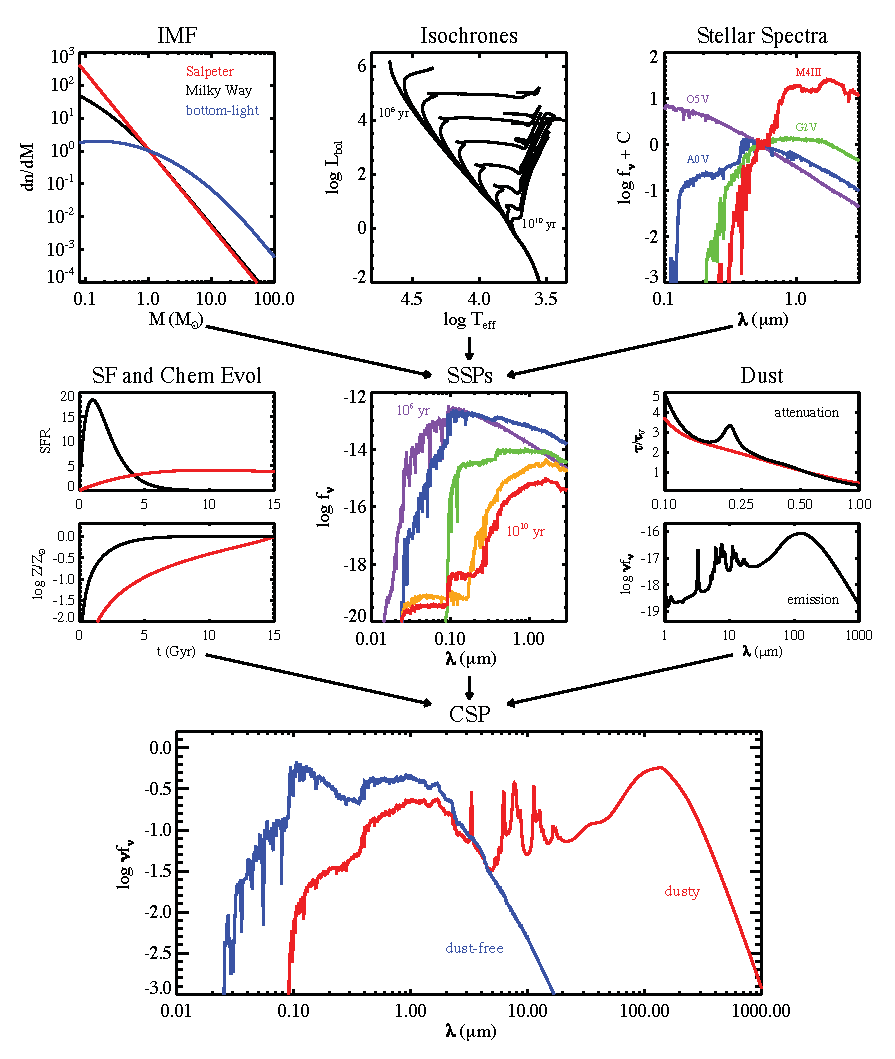
\includegraphics[width=1\textwidth]{sed_plot.pdf}
	  \caption[Schematic diagram of the steps in building composite stellar populations from \citet{Conroy:2013dk}.]{Schematic diagram of the steps in building composite stellar populations from \citet{Conroy:2013dk}. The ingredients for simple stellar populations on the top row; the initial mass function, stellar isochrones and stellar spectra -- are combined to make SSPs for different ages and metallicities. The SSPs are then combined based on a star-formation and metallicity history, before dust attenuation is applied (and the corresponding emissions then modelled) to make composite stellar populations. In the bottom plot, the blue spectrum represents the intrinsic stellar emission for the CSP while the red line shows how this spectrum changes due to dust.}
	  \label{fig:sed_plot}
\end{figure}

Most commonly used is a SFH which decays exponentially over some characteristic timescale, $\tau$, such that $\text{SFR}(t) \propto \exp(-t/\tau)$. More recently, it has been shown that rising star-formation models (e.g. negative $\tau$'s) are both a better a fit to the observed photometry of high-redshift galaxies \citep{Maraston:2010dl} and a better representation of the theoretical predictions from simulations \citep{2011MNRAS.410.1703F,Dayal:2013jm}. Other simple single parametrisations have also been applied such as the `delayed' model ($\propto \frac{t}{\tau^{2}} \exp(-t/\tau)$). At high-redshift, there is also now evidence that the average SFH is best-fit by an increasing power-law form \citep{2011MNRAS.412.1123P,2015ApJ...799..183S} rather than previously assumed exponential form. Another novel approach to constructing plausible and accurate star-formation and metallicity history is that of \citet{Pacifici:2012fr}, whereby a large number of SFR and Z histories from semi-analytic models are used to construct a more set of realistic CSPs for fitting.

However the SFR and metallicity histories of models are parametrised, what is most important is that the chosen models can accurately represent the full dynamic range of observed galaxy photometry and give un-biased estimates of the stellar population properties we are interested in measuring. At $z > 3$, when the Universe is less than $\sim 2$ Gyr old, the upper limits on the possible stellar ages means that degeneracies introduced into SED fitting from the SFH alone are somewhat reduced \citep{2013A&A...549A...4S}.

Another critical assumption in the use of SPS modelling is the choice of initial mass function. Unfortunately, it is not possible to constrain the IMF from the integrated light of galaxies alone. There exist just too many degeneracies to make any useful constraints except for the most special circumstances.  Without direct measurements of the IMF in distant galaxies, we are limited to the assumption of a fixed and universal IMF based on measurements of the local IMF such as the canonical \citet{Salpeter:1955hz} or \citet{Chabrier:2003ki} and \citet{Kroupa:2001ki} functions. 

While the optical and near-infrared filters of \emph{Hubble Space Telescope} are ideally suited for selecting galaxies at high-redshift due to the position of the redshifted Lyman break at $4 < z < 7$, they are not well-suited for deriving accurate stellar population properties such as stellar mass. This is because the rest-frame UV continuum probed by these filters is predominantly produced by young stars so is dominated by recent star-formation and (as mentioned in Section~\ref{sec:intro-earlygal}) is particularly sensitive to dust attenuation. Mid-infrared observations from the IRAC camera \citep{Fazio:2004eb} aboard the \emph{Spitzer Space Telescope} have been essential to making reliable estimations of galaxy properties at high-redshift, especially the deep observations at 3.6 and 4.5 \micron{} made during \emph{Spitzer's} post-cryogenic mission (e.g. \citeauthor{Ashby:2013cc}~\citeyear{Ashby:2013cc}). By extending the observations to mid-infrared wavelengths, it means constraints on the rest-frame optical emission of (brighter) high-redshift galaxies out to $z \geq 7$ are now possible.

Probing the rest-frame optical emission however comes with its own potential pitfalls. At $z \geq 4$ the bright nebular emission lines (such as H$\alpha$, $[\text{O}\textsc{iii}]$ and $[\text{O}\textsc{ii}]$) are redshifted into the 3.6 and 4.5 \micron{} IRAC bandpasses, potentially contaminating the broadband fluxes and systematically biasing the SED fitting. Early studies of galaxy SEDs at high redshift suggested that the measured stellar masses and ages may be systematically over-estimated because of such contamination \citep{2009A&A...502..423S,2010A&A...515A..73S,Ono:2010ed}. Accounting for the effects of nebular emission in SED fits is therefore vital in making un-biased measurements of galaxy properties at high-redshift.

At the onset of the work undertaken in this thesis, constraints on galaxy stellar masses at $z \geq 4$ were limited either by the small samples \citep{Gonzalez:2011dn} with WFC3 observations, or the limiting depth of ground-based near-infrared observations \citep{Stark:2007gi} available at the time. However, a new generation of deep near-infrared surveys means that it may now be possible to make robust studies of galaxy stellar mass evolution over the first few billion years of galaxy evolution.

\section{The CANDELS survey}\label{sec:intro-candels}
Regions of the sky that have been well studied by the \emph{Hubble Space Telescope}, such as the GOODS fields \citep{2004ApJ...600L..93G}, have become increasingly valuable resources for studying the evolution of galaxies (and the growth and activity of super-massive black holes) through cosmic time. This advance is thanks to the ever-growing wealth of observations across the whole electromagnetic spectrum, regularly reaching the most extreme depth observed at any particular wavelength. However, the deep fields such as GOODS North and South cover only very small areas of the sky ($\sim 320$ arcmin$^{2}$ combined for Hubble data) and the extremely deep \emph{Hubble} Ultra Deep Field extending to only a small fraction of this. Such small fields can lead to large uncertainties in galaxy counts due to cosmic variance and also makes them poor for studying the brightest and most massive objects.

While the deep optical coverage from \emph{Hubble's} Advanced Camera for Surveys (ACS) has allowed the Lyman break selection of galaxies out to $z\sim6$ and provided rest-frame optical morphologies of lower redshift galaxies, in order to extend this analysis to greater redshifts requires near-infrared observations of comparable depth to those existing at shorter wavelengths. Near-infrared surveys reaching to depths of $H_{160} \simgreat 26$ \emph{were} possible with the NICMOS camera, but were severely limited by the survey efficiency of the instrument with respect to its optical counter-part, ACS. The GOODS NICMOS Survey (GNS, \citeauthor{Conselice:2011ia}~\citeyear{Conselice:2011ia}) observed parts of the GOODS North and South fields to a depth of $H_{160} \sim 26.5$ (cf. $V_{606} = 27.8$, \citeauthor{2004ApJ...600L..93G}~\citeyear{2004ApJ...600L..93G}). Surveying 45 arcmin$^{2}$ to this depth in just one single filter required 180 orbits of Hubble observations. Clearly, extending such a survey to more filters and significantly greater areas was not feasible with the existing facilities. Furthermore, using ground-based facilities, the depths required to detect all but the brightest sources are just not possible, even with the largest 8m+ telescopes. 

\begin{figure}[hbt!]
	\centering
	\includegraphics[width=0.8\textwidth]{hst_efficiency.png}
	\caption[Discovery efficiency (defined as the field of view area multiplied by the system throughput) of the Hubble Space Telescope detectors.]{Discovery efficiency (defined as the field of view area multiplied by the system throughput) of the Hubble Space Telescope detectors. The order of magnitude increase in efficiency at near-IR wavelengths from NICMOS (orange dashed line) to WFC3 (solid dark blue line) is well illustrated. Credit: STScI/Space Telescope Science Institute}
		\label{fig:hst_efficiency}
\end{figure}

Thankfully, the greatly improved capabilities of the Wide Field Camera 3 (WFC3), installed in \emph{Hubble} as part of the final service mission, such a task was made considerably more feasible. The stark increase in efficiency at infrared wavelengths is illustrated in Figure~\ref{fig:hst_efficiency}. Furthermore, for equivalent exposures and signal-to-noise, the limiting magnitude of the WFC3/IR is up to $\sim 1$ magnitude fainter than that of NICMOS.

The CANDELS project (Cosmic Assembly Near-infrared Deep Extra-galactic Legacy Survey) leverages the new infrared capabilities to make observations which are both deeper and more extensive than previously available for the key legacy fields. Awarded 902 orbits of \emph{Hubble} time, CANDELS represents the largest HST project in its history. The final survey program involved observations of five key extra-galactic survey fields -- GOODS South, GOODS North, the extended Groth strip (EGS), the UKIDSS Ultra Deep Survey (UDS) and the COSMOS field -- with observations of these fields split into two distinct tiers. 

The first (and deepest) of these tiers, hereafter CANDELS/Deep, is primarily comprised of observations over parts of the GOODS North and South (totalling 120 arcmin$^{2}$) to a depth of $\sim 13$ Hubble orbits. The second shallower tier (CANDELS/Wide) consists of observations over all five fields with $\sim 2-3$ orbits per tile and covering 668 arcmin$^{2}$ to a depth comparable or greater than that in the GNS.

The first deep field completed was the GOODS South field and is the basis for the majority of the analysis undertaken throughout this thesis. Full details of this dataset can be found in \citet{Guo:2013ig}, including the data reduction and homogenisation of the respective space and ground-based ancillary data. 

In the context of the many outstanding questions in galaxy formation and evolution, the CANDELS survey set out with a wide range of primary scientific goals in four key areas:

\begin{enumerate}
		\item \emph{Cosmic Dawn}: the formation and early evolution of galaxies ($z > 4$)
		\item \emph{Cosmic High Noon}: the peak of star-formation and AGN activity ($1 < z < 3$)
		\item Ultraviolet Observations: Hot stars at $1 < z < 3.5$
		\item Supernovae: Standardizable candles beyond $z\sim1$
\end{enumerate}

It is the first of these areas in which the goals of this thesis lie.

%\begin{quotation}
%	``CD1	\quad Improve constraints on the bright end of the galaxy LF at $z \approx 7$ and 8 and make $z \approx 6$ measurements more robust.
%Combine with WFC3/IR data on fainter magnitudes to constrain the UV luminosity density of the universe at the end of the reionization era
%	
%	CD2 \quad Constrain star formation rates, ages, metallicities, stellar masses, and dust contents of galaxies at the end of the
%reionization era, $z \approx 6$ --10. Tighten estimates of the evolution of stellar mass, dust, and metallicity at $z = 4$-- 8 by combining WFC3 data with very deep Spitzer IRAC photometry"
%\end{quotation}

\section{Thesis Outline}

The aim of this thesis is to improve our understanding of the growth of galaxies during the first few billion years of cosmic history through studying their stellar mass, star-formation and merger history in details not previously possible at this epoch. Alongside this, we also aim to better understand the role that galaxies played in the epoch of reionization and place new constraints on their ability to power reionization.

{\bf Chapter~\ref{ch:smf}} makes use of the deep multi-wavelength data of the CANDELS GOODS South field to investigate the evolution of the stellar mass function at redshift $z\sim4$ and above. In addition to the stellar masses we make estimates of the galaxies' star-formation rates to study the evolution of the specific star-formation rates and star-formation rate function with redshift. As part of this chapter we also undertake extensive tests to explore the reliability of photometric selection for galaxies at high-redshift in comparison to a more traditional Lyman-break selection.

{\bf Chapter~\ref{ch:mergers}} then investigates the major merger rates of galaxies at $z > 2$ in the GOODS South field. We study the photometric close-pair statistics using a new approach which corrects for chance line-of-sight pairs using the photometric redshift probability distributions. By applying this method to a sub-sample of the available CANDELS data, we aim to show that it is now possible to study the merger properties of mass selected galaxies as far back as $z\sim6$.

In both Chapters~\ref{ch:smf} and ~\ref{ch:mergers} we make use of semi-analytical and hydrodynamical models to compare our new observations with the predictions of theoretical models at high-redshift.

{\bf Chapter~\ref{ch:reionization}} studies the current constraints on the potential for galaxies to provide sufficient numbers of ionizing photons to power reionization. Using the latest observations of the galaxy rest-frame UV luminosity and stellar mass functions at high redshift (including the results of Chapter~\ref{ch:smf}) and their UV continuum colours, we use extensive SED modelling to make new estimates of the ionizing emissivity during the epoch of reionization.

In the final chapter we discuss the conclusions drawn from the work done in this thesis and explore how future work can build on these results.
%% %% End of file...  %%
